\documentclass[letterpaper,10pt]{article}

\usepackage{titling}
\usepackage{listings}
\usepackage{url}
\usepackage{setspace}
\usepackage{subfig}
\usepackage{sectsty}
\usepackage{pdfpages}
\usepackage{colortbl}
\usepackage{multirow}
\usepackage{multicol}
\usepackage{relsize}
\usepackage{amsmath}
\usepackage{wasysym}
\usepackage{fancyvrb}
\usepackage{amssymb}
\usepackage{ifsym}
\usepackage{amsmath,amssymb,amsthm,graphicx,xspace}
\usepackage[titlenotnumbered,noend,noline]{algorithm2e}
\usepackage[compact]{titlesec}
\usepackage{XCharter}
\usepackage[T1]{fontenc}
\usepackage{tikz}
\usetikzlibrary{arrows,automata,shapes,trees,matrix,chains,scopes,positioning,calc}
\tikzstyle{block} = [rectangle, draw, fill=blue!20, 
    text width=2.5em, text centered, rounded corners, minimum height=2em]
\tikzstyle{bw} = [rectangle, draw, fill=blue!20, 
    text width=4em, text centered, rounded corners, minimum height=2em]

\definecolor{namerow}{cmyk}{.40,.40,.40,.40}
\definecolor{namecol}{cmyk}{.40,.40,.40,.40}

\let\LaTeXtitle\title
\renewcommand{\title}[1]{\LaTeXtitle{\textsf{#1}}}


\newcommand{\handout}[5]{
  \noindent
  \begin{center}
  \framebox{
    \vbox{
      \hbox to 5.78in { {\bf ECE356: Database Systems } \hfill #2 }
      \vspace{4mm}
      \hbox to 5.78in { {\Large \hfill #4  \hfill} }
      \vspace{2mm}
      \hbox to 5.78in { {\em #3 \hfill} }
    }
  }
  \end{center}
  \vspace*{4mm}
}

\newcommand{\lecture}[3]{\handout{#1}{#2}{#3}{Lecture #1}}
\newcommand{\tuple}[1]{\ensuremath{\left\langle #1 \right\rangle}\xspace}

\addtolength{\oddsidemargin}{-1.000in}
\addtolength{\evensidemargin}{-0.500in}
\addtolength{\textwidth}{2.0in}
\addtolength{\topmargin}{-1.000in}
\addtolength{\textheight}{1.75in}
\addtolength{\parskip}{\baselineskip}
\setlength{\parindent}{0in}
\renewcommand{\baselinestretch}{1.5}
\newcommand{\term}{Winter 2018}

\singlespace


\begin{document}

\lecture{ 13 --- File Organization }{\term}{Jeff Zarnett}

\section*{File Organization}

Recall from earlier that there were a few different file organization options we could choose~\cite{fds}:

\begin{enumerate}
	\item \textbf{Heap File}: An unordered file where new records are just appended to the end.
	\item \textbf{Sorted File}: The file is ordered based on a particular field (the sort key).
	\item \textbf{Hashed File}: The file is ordered based on the result of a hash function applied to a particular field.
	\item \textbf{B-Tree File}: The file is organized using a B-tree structure.
\end{enumerate}

We did not go into the details of the options earlier, but we will now be able to do so. Under most circumstances one relation corresponds to one file. However, multiple relations can be in the same file if desired. To start with, we will just have one relation in a file. 

Remember that these file organizations are not affected by whether records are of fixed or variable length. Similarly, whether spanned records is allowed or not does not affect the file organization. Those sorts of consideration are about how to pack records into a block; this is about the order of the records. The first $k$ records may be stored in the first block, but which records are the first $k$?

\subsection*{Heap File} 

The simplest way to order records is: don't order the records! The heap file has no inherent organization, although some (weak) idea of ordering may exist in the sense that records appear in the file in the order in which they are inserted. However, there is no guarantee about that, and if that is the behaviour it is an implementation detail and should not be relied upon. 

This strategy makes insertion efficient -- just tack this on to the end of the file, a constant time ($O(1)$) operation . If a new block is needed, allocate that new block and write it to disk. If not, the last block of the file is read, modified, and written. That part is simple. However, searching for a record is more difficult, because the file is not ordered in any way. Thus, we would have to perform a linear search ($O(n)$) over all records. To find one individual record in the relation it be necessary to examine, on average, half of the entries (assuming that all requests are equally likely). If the element is not in the file at all then we have to examine all the elements, and it was all for nothing anyway~\cite{fds}. 

To delete a record, we need to first search for the record (linear search), then rewrite the block that it is in. Ultimately after enough deletions there will be multiple partially-full blocks, leading to wasted space. Thus, compaction of some sort will eventually need to take place which moves the records around to fill in these holes.

An update has all the problems we've discussed before. We must linear search to find the record(s) to the updated.  It may lead to reorganization of a block or having to move the file to a different block, treating it as if it is an insertion and deletion.  

Heap organization throws into the light the idea that the file structure has performance implications: that is, no matter what we choose, it will mean some operations are faster at the expense of other operations. Heap organization means that insertion is fast but reading, updating, and deleting are slower. This seems incongruous with our usual expectations of what databases are for. Normally we would expect retrieval to be the most common operation, right?

\subsection*{Sorted File}

Long, long ago in an introductory programming course you learned about sorting, and perhaps more importantly, the idea that if you are going to search your data (more than once anyway). Usually in such sorting exercises you are asked to sort a bunch of integers. Integers have nice properties including a logical, simple ordering, and you can tell quickly at a glance if the array has been sorted correctly or not. In a sequential file, we will sort the records based on one particular attribute from start to end.

The field that we sort the file on is called the \textit{ordering field}, and if it is a  unique key then it is called an \textit{ordering key}~\cite{fds}. It does not have to be the primary key. A search that is on the ordering field is quite efficient. Suppose employees have sequential unique employee ID numbers and that is the ordering key in the database. If the goal is to find all employees with an ID less than 385, the data is sequential in all the blocks and that is convenient.

To find an individual record we can use a binary search ($O(\log n)$) which is for finding a record as well as update and deletion as discussed earlier. We are likely to access $\log_{2}(n)$ blocks, whether or not we find what we are looking for.

A simple sequential organization looks like~\cite{dsc}:

\begin{center}
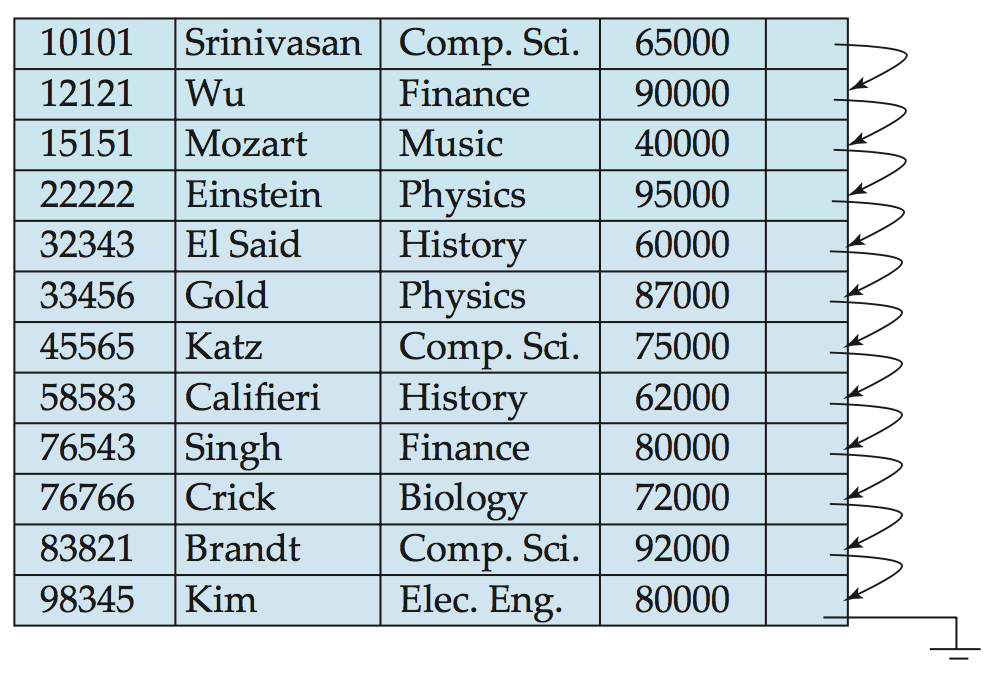
\includegraphics[width=0.4\textwidth]{images/sequential}
\end{center}

In looking at this diagram we can see that they are sorted by some sort of integer ID (the leftmost column) in ascending order. And yet, there is a pointer in the rightmost column pointing to the next record and the next and the next. What purpose would that serve? It is for efficiency reasons, of course. 

It can be difficult to maintain the physical ordering of the data because every insertion, deletion, and perhaps update requires a lot of moving records around. So we could potentially relax the constraint of having to keep all the records in order at all times. Instead, we could temporarily have the following physical layout~\cite{dsc}:

\begin{center}
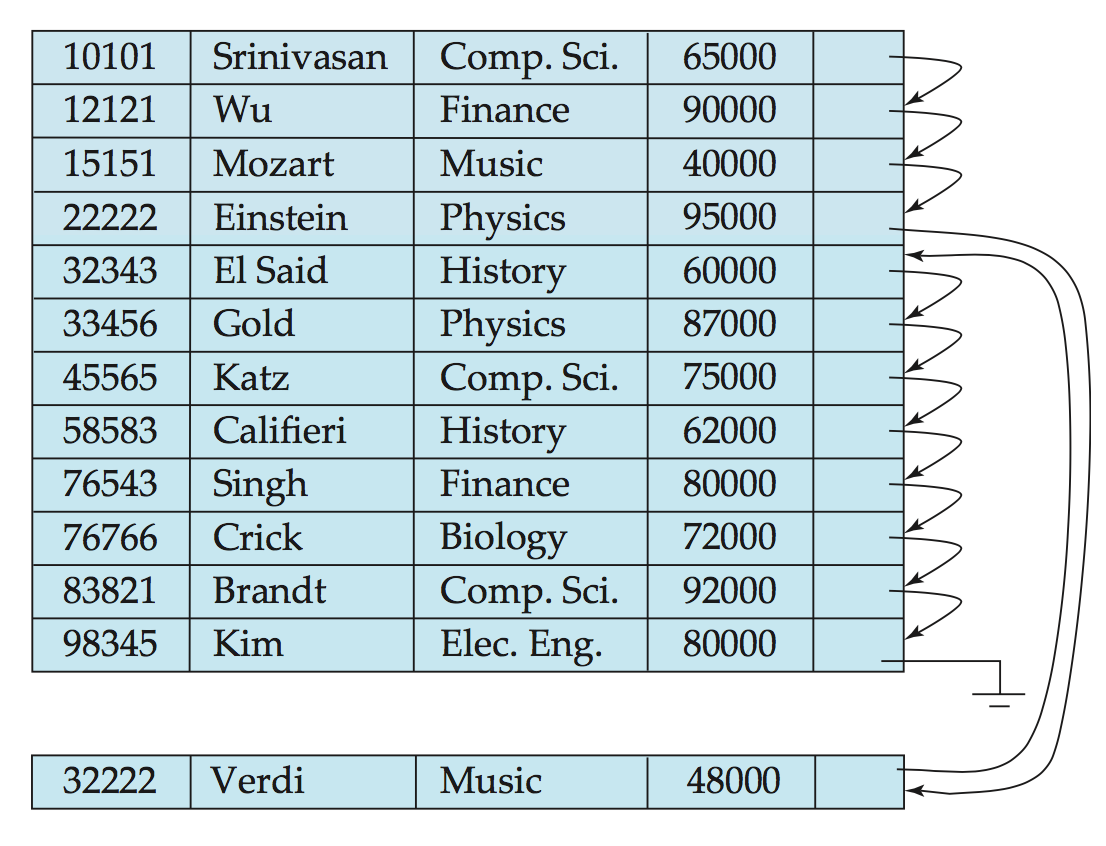
\includegraphics[width=0.45\textwidth]{images/sequential-2}
\end{center}

If the insertion we are doing goes at the end of the file such as in the example an ID of 99001 is inserted, then the file maintains its sequential order. If there is a free space in the block where the record belongs, then we can put the record in the correct block although it is out of order. If, as in the case shown above, the block is full then we need to place the new record somewhere else. For that there is often an \textit{overflow block} where records that do not fit into their normal locations go. 

Deletion is the mirror image of insertion. If we deleted the record at the very end of the file, there is nothing special to maintaining order. If the record being deleted is in an overflow block, that makes the order more sequential rather than less. If the record inside a block is being deleted, such as the record with ID 58583 then the pointer from record 45565 would just be updated to point to 76543 and that would suffice. The empty space would be noted for the future. 

If this continues over time, the file loses its sequential ordering as more and more records end up in overflow blocks. The file becomes less and less sequentially organized, meaning it resembles the heap file more and more. Eventually the file must be reorganized which sorts the records based on the sequential order again, potentially moving a large number of records to get them into the order where they belong. Because this is a potentially expensive operation, it would likely only be done when the system is not busy and when there are enough records out of order that it makes sense to do this. 

\subsection*{Hashed File}

A hashed file works very much like the sorted file, except, instead of the sorting key being a number, a hashed value is used instead. The hash technique can allow for fast access to records. The hash field is often the key. On its own that does not sound any different than the sorted file, but the ``magic'' in the use of the hash function is that instead of the ID being just a number, the hashed value tells us the address of the disk block in which the record is stored~\cite{fds}. So instead of having to binary search to find the record with ID 99901, we could instead compute the hash value and find out that it is in block $x$ and then go directly there.

We will take a short digression to cover the subject of hashing, actually. Chances are you covered this in a data structures and algorithms course, but it was probably in the context of hashing a value to find what index in the array to insert a particular element. That is \textit{internal hashing}, which we will quickly review, but hashing can be much more.

If you implement a hash table simply, there is an array with $M$ ``slots'' and then the hash function turns a particular value into an integer between $0$ and $M-1$. The hash function can be as simple as some integer field modulo $M$. That algorithm will work but probably does not provide ``nice'' properties to the hash function, or its output. If you don't have an integer field you want to hash (no ``id'' or other such field), don't despair. You can simply interpret everything as an integer if you want! It's all ones and zeros when you drill down to it and you can just pretend this string or double or binary data is an integer number and problem solved~\cite{fds}.

It is more likely that you actually want a hash function that has some better properties. A \textit{folding} hash function does some arithmetic operations -- add up some numbers, reverse some positions, move blocks around, the like, and usually a modulo operation is the last step to get everything cut down to the right size.

Regardless of how the hash function is calculated, we need to deal with the fact that two input values will eventually produce the same output value. This is called a \textit{hash collision} and it is super common, because the range of output addresses is very often smaller than the range of input.\footnote{There are ``perfect'' hash functions that don't produce collisions, incidentally.} You may, for example, have an array that can contain 4096 elements, but if the input values are a range from $0$ to $2^{16}$ then there will definitely be collisions. That itself is not a bad thing, as long as we have a way to handle this situation. We can apply three major approaches for how we handle hash collisions from~\cite{fds}. 

The first is \textit{Open Addressing} -- simply go to the next open space if we must. Suppose the hash function computes $n$ but there is already an element stored at that position. Then just go to position $n+1$ and put it there (if possible, otherwise go to $n+2$, etc). This is simple, but it can lead to clustering, where a bunch of elements are close together.

The next strategy is \textit{chaining}. In this case, we have overflow locations. If there is a collision, we put the new item in an empty space and put a pointer from one element to the next. 

The third strategy is a second hash function (\textit{multiple hashing}) that is run if we have a collision to differentiate. We could have a third, fourth, etc. function but as one point we will default to open addressing because we will have no other choice.

A goal of hashing is to distribute the records relatively evenly across the address space so that we do not have too many collisions, but also do not have too much empty space. Ideal is something like 70-90\% full; and if we need to make the table bigger (or smaller), then we do so. If $M$ is a prime number, we get good distributions, although other technical constraints like the hashing algorithm may mean a power of 2 is best~\cite{fds}.

With the review of internal hashing aside, we should take a look at external hashing, which is what we need for files on disk. Instead of viewing the data storage as an array  where we can store one element, instead we have buckets that hold multiple records... which is exactly what you should expect given that we have already talked about blocks. Then, the hashing function produces a bucket (block) number, and then from there we can get to the actual record by looking in the header for the block. 

This does ameliorate some of the collision problem; if we have multiple records that produce the same hash value it's not a big deal because they can go in the same bucket. Nevertheless, we need to still be concerned about what happens when buckets are full, and as you might expect the solution for this will be overflow blocks. 

Still, all the hashing we have covered so far is \textit{static hashing}, that is to say, we have a fixed number of buckets. That is not suitable for our purposes a database where files will need to grow as the amount of data in the tables increases (or not be allocated as ridiculously large and mostly empty in the first place). If most buckets are close to full, we could simply add more buckets and then use a new hashing function (with the new maximum size) to reassign all the items to their new buckets, but this sort of global reorganization is very very slow~\cite{fds}.

The following image shows how a strategy of buckets with overflow buckets may look (simplified)~\cite{fds}:

\begin{center}
	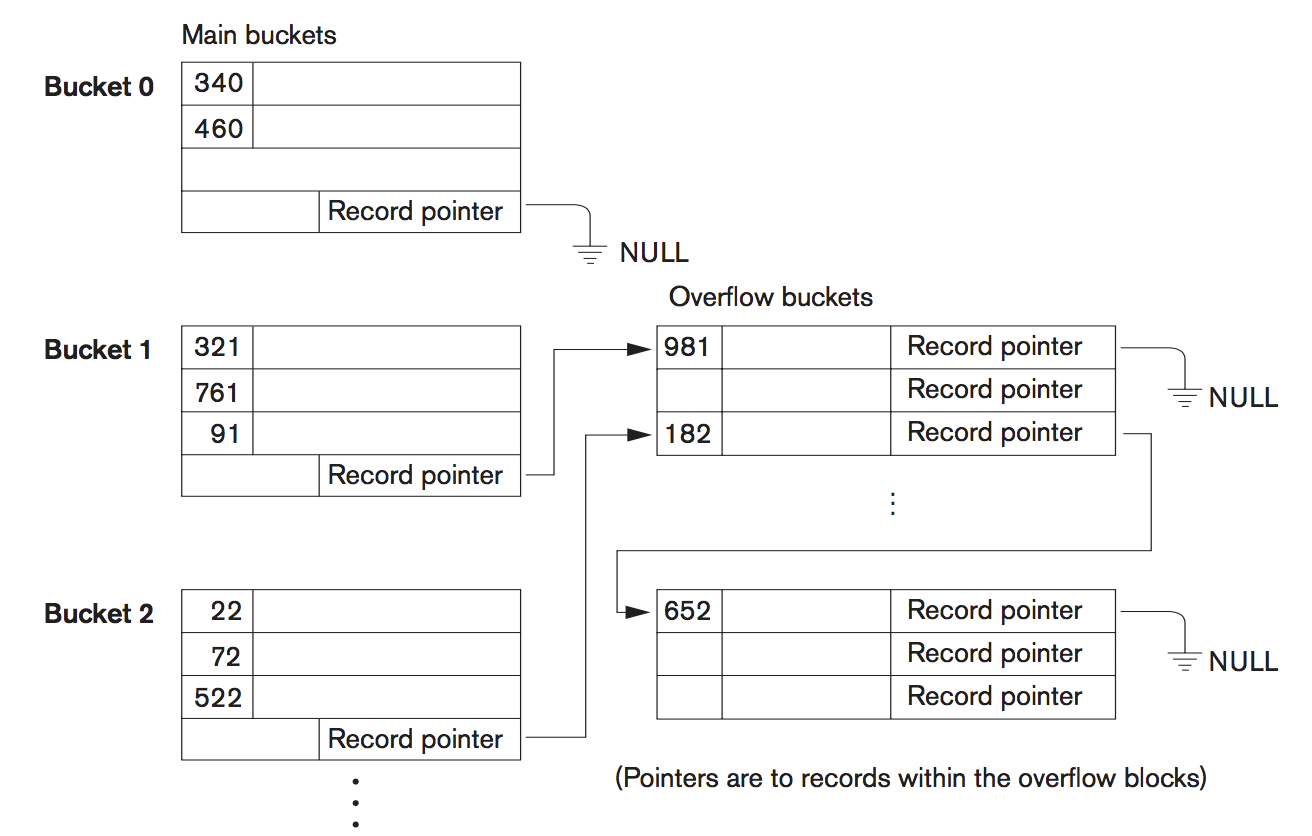
\includegraphics[width=0.75\textwidth]{images/overflow-buckets}
\end{center}

Much better would be a hashing function that permits dynamic file expansion. That is to say, the file grows and shrinks as needed based on the amount of data that is in the file.

The first approach is \textit{extendible hashing} -- an access structure is stored in addition to the file. The access structure is an array of $2^{d}$ bucket addresses, where $d$ is the global depth of the directory. The first $d$ bits of a hash value are the index into the array to determine which element of the array is selected; the array element is the bucket in which the corresponding entry is stored. What makes this dynamic is that there may be duplicates in the array. Local depth $d'$ (``Dee prime'') specifies the number of bits on which the local bucket contents are based~\cite{fds}. The hash value will usually be interpreted as a sequence of bits.

This may make more sense if displayed visually~\cite{fds}:

\begin{center}
	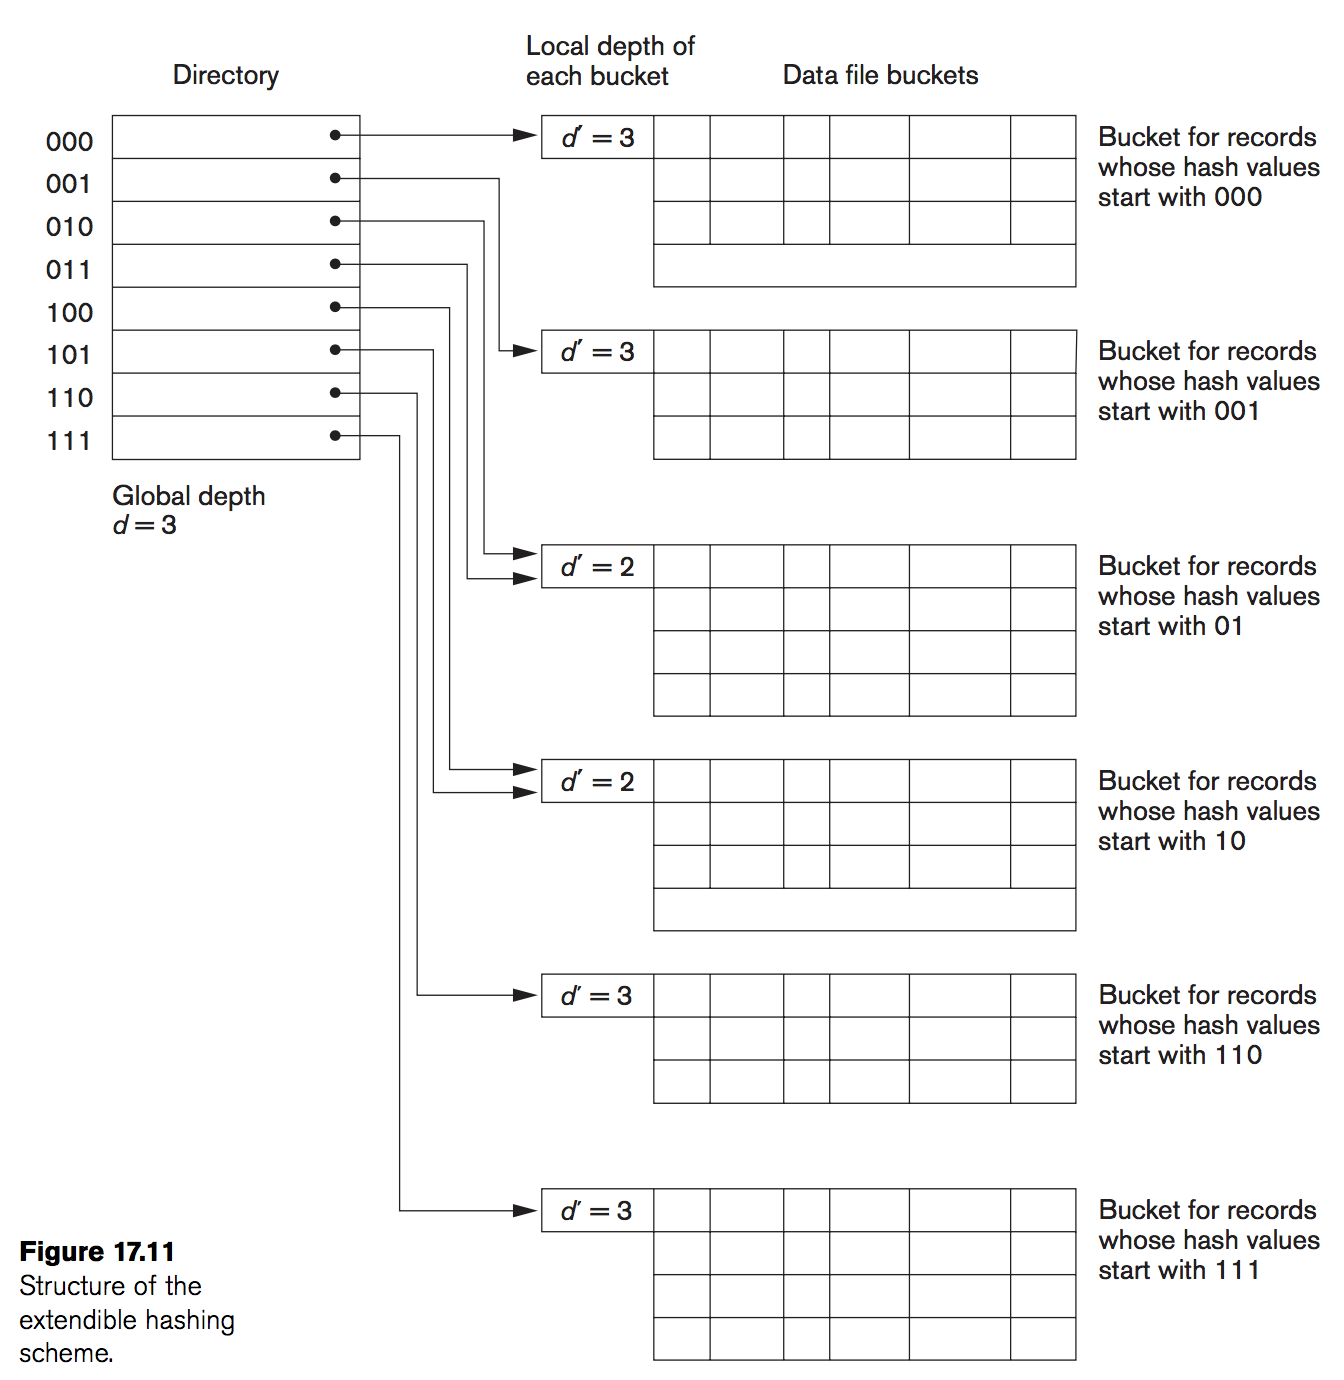
\includegraphics[width=0.75\textwidth]{images/extendible-hashing}
\end{center}

Suppose we are running out of space: that means that a bucket whose depth $d'$ is equal to $d$ has become full and is now overflowing. That would mean we increase the value of $d$ which doubles the number of buckets. A quick example of bucket splitting from~\cite{fds} in the previous diagram would be what happens if the bucket whose hash values start with 01 becomes full. At that point we need to split the records up between those that start with 010 and those that start with 011. Those are now two distinct buckets with $d'$ of 3. That is fine, because $d'$ can range from 1 to $d$ (inclusive) but no higher.  

If one of the buckets with $d'$ equal to $d$ becomes full, then we need to split those as well and the size of $d$ must increase (in this example, to 4). Alternatively, if $d'$ is smaller than $d$ for all buckets (which could happen after enough deletions occur), we could potentially decrease $d$ by 1~\cite{fds}.

Extendible hashing is great because it allows the file to grow and shrink as is appropriate with the amount of data that is in the file. As things get close to full, we just create a new bucket (or several buckets) and the rate of collisions falls again. If we have to split a bucket, then a relatively small number of records need to be moved, because it is only some of the records in the bucket being split that need to go to the new bucket. 

If we have to increase the value of $d$ then we have a potentially larger and more painful reorganization, but we probably won't lose any sleep over that. Why not? When $d$ is small, the total number of records in the system is not very large so the time to move all of them (worst case) is not very big. For example, if $d$ is 3, if the table is completely full, there are $2^{3} = 8$ buckets. Not very many. If $d$ is large then increasing it is very rare. If $d$ is 16 there are $2^{16} = 65~536$ buckets and it takes a long time to fill them up. Ah, the power of exponential growth.

% Dynamic Hashing?
% Linear Hashing?

There exist other hashing strategies, dynamic and linear hashing, notably, but we will not examine them at the moment.

\subsection*{B-Trees}

We will assume that everyone is familiar with B-Trees from a data structures and algorithms course (and perhaps a review from an operating systems course...). We will actually look into B-Trees in more detail when we talk about the idea of indexing. But theoretically we could use B-Trees to store the data in a way that very much resembles how operating systems store files on disk.


\subsection*{Multiple Record Types}

Everything else so far has assumed that each type of record has its own file. That is not a requirement; it is possible to keep multiple types of record in the same blocks. This could speed up join queries that go over both tables but perhaps slow down other queries. To make this work we need a differentiator, of some sort, to tell us what kind of record each record is, and that is generally a simple field of some sort.

In a similar but less extreme variation, we could put tables that we know to be related next to one another on disk which could potentially reduce the amount of effort to read and write related records.

\bibliographystyle{alphaurl}
\bibliography{356}


\end{document}
